\documentclass[12pt, a4paper]{article}

\usepackage[utf8]{inputenc}
% Limit the page margin to only 1 inch.
\usepackage[margin=1in]{geometry}

%Imports biblatex package
\usepackage[
backend=biber,
style=alphabetic
]{biblatex}
%\addbibresource{../../mth342.bib}

% Enables the `align' environment.
\usepackage{amsmath}
% Provides useful environments, such as:
% - \begin{proof} ...\end{proof}
\usepackage{amsthm}
\usepackage[most]{tcolorbox}

\newtheorem*{proposition}{Proposition}
\theoremstyle{definition}
\newtheorem*{definition}{Definition}

% Enables using \mathbb{}, for example \mathbb{N} for the set of natural numbers.
\usepackage{amssymb}

% Allows using letters in enumerate list environment. Use, for example:
%\begin{enumerate}[label=(\alph*)]
% ...
%\end{enumerate}
\usepackage[inline]{enumitem}

% Enable importing external graphic files and provides useful commands, like \graphicspath{}
\usepackage{graphicx}
% Images are located in a directory called "images" in the current directory.
\graphicspath{{./images/}}

% Make links look better by default.
% See: https://tex.stackexchange.com/questions/823/remove-ugly-borders-around-clickable-cross-references-and-hyperlinks
\usepackage[hidelinks]{hyperref}
\usepackage{xcolor}
\hypersetup{
	colorlinks,
	linkcolor={red!50!black},
	citecolor={blue!50!black},
	urlcolor={blue!80!black}
}

% Code Listings. Source:
% https://stackoverflow.com/questions/3175105/inserting-code-in-this-latex-document-with-indentation
\usepackage{listings}
\usepackage{color}

\definecolor{dkgreen}{rgb}{0,0.6,0}
\definecolor{gray}{rgb}{0.5,0.5,0.5}
\definecolor{mauve}{rgb}{0.58,0,0.82}

\lstset{frame=tb,
	language=Java,
	aboveskip=3mm,
	belowskip=3mm,
	showstringspaces=false,
	columns=flexible,
	basicstyle={\small\ttfamily},
	numbers=none,
	numberstyle=\tiny\color{gray},
	keywordstyle=\color{blue},
	commentstyle=\color{dkgreen},
	stringstyle=\color{mauve},
	breaklines=true,
	breakatwhitespace=true,
	tabsize=3
}

\newcommand{\prob}{\text{P}}
%\newcommand{\complement}{\mathsf{c}}

\title{Lecture 04: MATH 342W: Introduction to Data Science and Machine Learning}
\author{Sergio E. Garcia Tapia\thanks{Based on lectures of Dr. Adam Kapelner at Queens College.
		See also the \href{https://github.com/kapelner/QC_MATH_342W_Spring_2025}{course GitHub page}.}}
\date{February 6, 2025 (last updated \today)}

\begin{document}
	\maketitle
	
	\subsection*{Recap}
	Let's begin by recapping some concepts. When studying a phenomenon in real life,
	there is a response variable $y$ related to other quantities of interest:
	\begin{align*}
		y &= t(z_1,\ldots,z_t)\\
		&= f(x_1,\ldots,x_p) + \delta\\
		&=h^*(x_1,\ldots,x_p) + \epsilon\\
		&=g(x_1,\ldots,x_p) + e
	\end{align*}
	\begin{itemize}
		\item $z_1,\ldots,z_t$: The ``true" drivers or causal information for the phenomenon of interest.
		\item $x_1,\ldots,x_p$: Features (also known as predictors, independent variables,
		covariates, etc) that are proxies to the $z$'s.
		\item $f$: ``best" function that maps the features to the response $y$.
		\item $h^*$: ``best" candidate function in our hypothesis set $\mathcal{H}$.
		\item $\mathcal{H}$: Set of candidate functions of some functional form that we choose to
		approximate $f$.
	\end{itemize}
	
	There are three types of errors:
	\begin{enumerate}[label=(\roman*)]
		\item \emph{Ignorance error} $\delta = t - f$: The error incurred because the predictors
		$x_1,\ldots,x_p$ cannot possibly capture all the information implied by the
		true drivers $z_1,\ldots,z_t$. We can decrease $\delta$ by increasing the
		number of features we use (increase $p$).
		\item \emph{Misspecification error} $\epsilon-\delta=f-h^*$: Error incurred by choosing
		a hypothesis set $\mathcal{H}$ that may not correctly capture the functional behavior of $f$.
		We can decrease it by choosing a more expansive $\mathcal{H}$.
		\item \emph{Estimation error} $h^*-g$: Error incurred by not having enough data
		(i.e., enough examples). We can decrease it by improving $\mathcal{A}$ (the algorithm)
		or by increasing $n$ (using more data).
	\end{enumerate}
	\subsection*{The Null Model, $g_0$}
	What if we only have outputs, and have no features, so that the tuples in $\mathbb{D}$
	consist only of the values of $\mathbf{y}$? This is called $g_0$, \textbf{the null model}.
	If $\mathcal{Y}=\{0, 1\}$, then we can define
	\begin{align*}
		g_0 := \text{Mode}[\mathbf{y}]
	\end{align*}
	Here $g_0$ is a constant function from $\mathcal{X}$ to $\mathcal{Y}$. For example,
	if the most frequent response is $0$, the $g_0$ will always predict $0$ regardless
	of its input.
	
	Note that $g_0$ is the best we can do if we do not have any features. However, the concept
	of a null model is useful even if we do have features because we can use it as our reference
	for performance. For example, suppose that $\mathcal{Y}=\{0, 1\}$, and that the responses in our
	historical data $\mathbb{D}$ have $24\%$ $1$'s and $76\%$ $0$'s. Then the mode is $0$,
	and the null model $g_0$ will always predict zero. Therefore, $g_0$ will misclassify $24\%$
	of the data in the training sample. Note that $g_0$ does not take any predictors into account,
	so if our predictors $x_1,\ldots,x_p$
	are chosen carefully, we should be able to beat $g_0$ (that is, the \textbf{misclassification error}
	should be smaller). If our misclassification error is ever higher than $g_0$, then either
	our algorithm $\mathcal{A}$ is bad, or our features are poor proxies to the $z$'s.
	
	\subsection*{Extending the Threshold Model}
	Recall the threshold model. Given $f:\mathcal{X}\to\mathcal{Y}$ that best approximates a true
	phenomenon $t$, where $\mathcal{X} = \mathbb{R}$ and $\mathcal{Y} = \{0, 1\}$, we have
	historical data $\mathbb{D}$ as in Figure~\ref{fig:threshold-model}.
	\begin{figure}
		\centering
		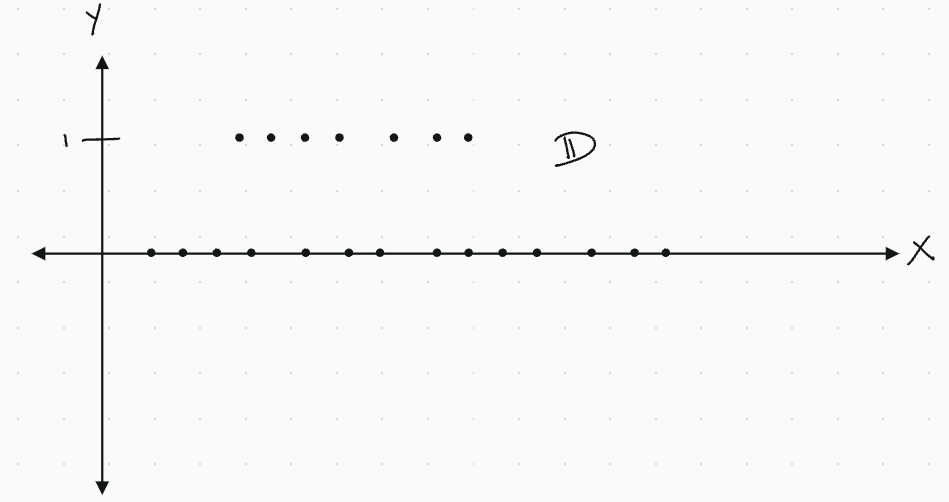
\includegraphics[width=0.6\textwidth]{threshold-model}
		\caption{A plot of historical data $\mathbb{D}$, where $\mathcal{X}=\mathbb{R}$
		and $\mathcal{Y} = \{0, 1\}$.}
		\label{fig:threshold-model}
	\end{figure}
	Continuing with the binary response space $\mathcal{Y}=\{0, 1\}$, suppose now that
	we have 2 numeric features, so that $\mathcal{X}=\mathbb{R}^2$, as in
	Figure~\ref{fig:2d-threshold-model}.
	\begin{figure}
		\centering
		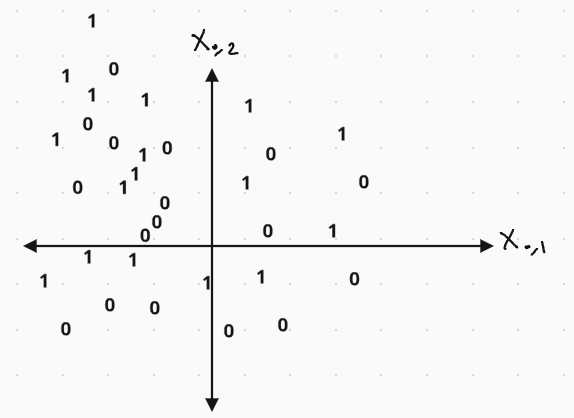
\includegraphics[width=0.6\textwidth]{2d-threshold-model}
		\caption{A plot of historical data $\mathbb{D}$, where $\mathcal{X}=\mathbb{R}^2$
			and $\mathcal{Y} = \{0, 1\}$.}
		\label{fig:2d-threshold-model}
	\end{figure}
	How can we extend the threshold model to two dimensions? Specifically, we need to come up
	with a hypothesis set $\mathcal{H}$ of functions that map each coordinate pair to $0$ or $1$.
	Recalling that $\mathcal{H}$ was made up of indicator functions with a parameter $\delta$
	in the case of the threshold model, one idea could be to have $\mathcal{H}$ consist of functions
	that are each a sum of two indicator functions, such as:
	\begin{align*}
		\mathcal{H} = \{\mathbb{I}_{x\geq \theta_2} + \mathbb{I}_{x\geq \theta_2}: \theta_1,\theta_2\in\mathbb{R}\}
	\end{align*}
	However, such functions don't map to $\mathcal{Y}=\{0, 1\}$, since they could have
	an output of $2$. Another idea is to use a product of indicator functions:
	\begin{align*}
		\mathcal{H} = \{\mathbb{I}_{x\geq \theta_1}\cdot \mathbb{I}_{x\geq \theta_2}: \theta_1,\theta_2\in\mathbb{R}\}
	\end{align*}
	While the functions in this $\mathcal{H}$ do map into $\mathcal{Y}$, we pay the
	price in high misspecfication error. By the way, $\theta_1$ and $\theta_2$ define
	what is referred to as a \textbf{parameter space}, and the number of parameters
	(in this case 2) is referred to as the \textbf{degrees of freedom}.
	
	A third idea is the following: we can draw a line through the data, as in Figure~\ref{fig:linear-model}.
	\begin{figure}
		\centering
		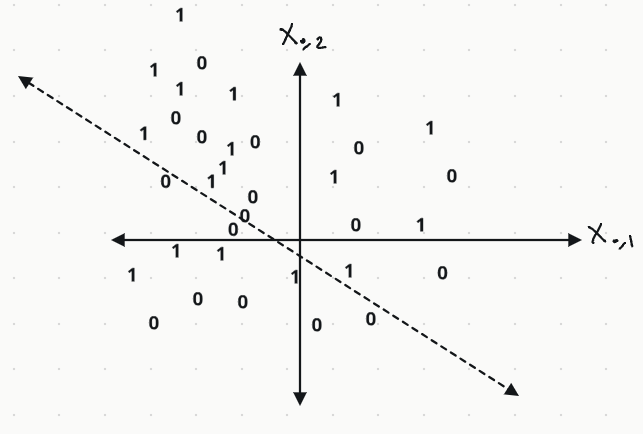
\includegraphics[width=0.6\textwidth]{linear-model}
		\caption{A linear model for the data in Figure~\ref{fig:2d-threshold-model}.}
		\label{fig:linear-model}
	\end{figure}
	A set $\mathcal{H}$ that captures this idea is
	\begin{align*}
		\mathcal{H} = \{\mathbb{I}_{x_2\geq \theta_1+\theta_2 x_1}: \theta_1,\theta_2\in\mathbb{R}\}
	\end{align*}
	This is called the \textbf{linear model}. Here, we say that if a point lies on or above the line,
	then the response should be 1; otherwise, 0.
	\subsection*{Perceptron}
	The \textbf{perceptron model} follows naturally from the linear model idea that we just
	described. We'll introduce it with a slight change of notation, using $w$ instead
	of $\theta$ for the parameters:
	\begin{align*}
		\mathcal{H} = \{\mathbb{I}_{w_0+w_1x_1+w_2x_2\geq 0}: w_0, w_1, w_2\in \mathbb{R}\}
	\end{align*}
	The $w_0$ term is the \textbf{bias} or \textbf{intercept}, and the $w_1$ and $w_2$ terms
	are the \textbf{feature weights}. Next, recall that we typically refer to $X$
	as an $n\times p$ matrix corresponding to $\mathbb{D}$:
	\begin{align*}
		X =\begin{bmatrix}
			\mathbf{x}_{\cdot, 1} & \cdots & \mathbf{x}_{\cdot, p}
		\end{bmatrix}
	\end{align*}
	where $\mathbf{x}_{\cdot, i}$ is our way of denoting the $i$th column vector of $X$,
	which consists of all possible values for the $i$th feature coming from $\mathbb{D}$.
	For the perceptron, we'll add another column to $X$, so we'll refer to it as
	\begin{align*}
		X = \begin{bmatrix}
			\vec{\mathbf{1}}_n & \mathbf{x}_{\cdot, 1} & \cdots & \mathbf{x}_{\cdot, p}
		\end{bmatrix},
		\quad \text{where }
		\vec{\mathbf{1}}=\begin{bmatrix}
			1\\
			1\\
			\vdots\\
			1
		\end{bmatrix}
	\end{align*}
	Here we use $\vec{\mathbf{1}}_n$ to denote a column of $1$'s.
	Hence, $X$ is now an $n\times (p+1)$ matrix. This extra column is for the \textit{intercepts},
	so it corresponds to the intercept term $w_0$. Now, the \textbf{perceptron learning algorithm}
	$\mathcal{A}$ tries to do the following:
	\begin{align*}
		\mathcal{A}: \mathbf{w}_{*}
		= \underset{\vec{\mathbf{w}}\in \mathbb{R}^3}{\text{argmin}}
		\left\{\sum_{i=1}^{n}\mathbb{I}_{\hat{y}_i\neq y_i}\right\},
		\quad
		\text{ where } \hat{y}_i = \mathbb{I}_{\mathbf{w}\cdot \mathbf{x}\geq 0}
	\end{align*}
	where the sum is the \textit{misclassification error}. In other words, the algorithm attempts to find
	the parameters for a line that minimize the misclassification error. There is no analytic solution
	to this.
	\begin{tcolorbox}[breakable]
		\begin{definition}[Perfect linear separability]
			Given historical data $\mathbb{D}$, there is perfect linear separability if
			there exists $\mathbf{w}$ such that
			\begin{align*}
				h(\mathbf{x}) = \mathbb{I}_{\mathbf{w}\cdot \mathbf{x}\geq 0}
			\end{align*}
			has no misclassification errors for all $\mathbf{x}\in \mathbb{D}$.
		\end{definition}
	\end{tcolorbox}
	See Figure~\ref{fig:perfectly-linearly-sperable}.
	\begin{figure}
		\centering
		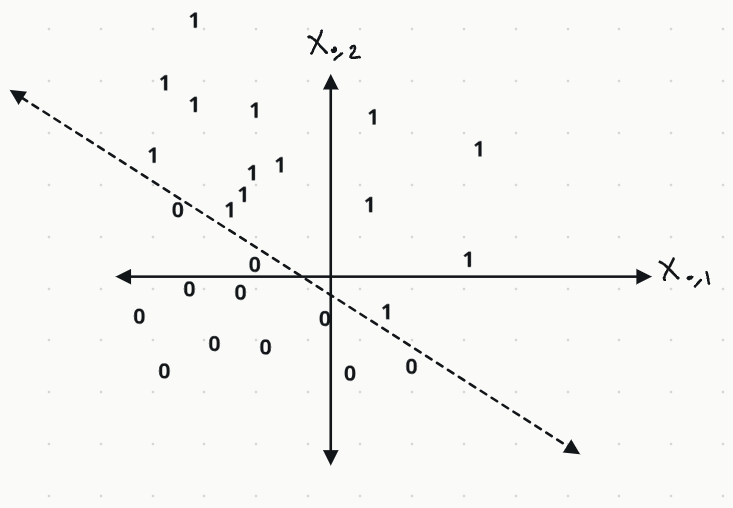
\includegraphics[width=0.6\textwidth]{perfectly-linearly-separable}
		\caption{An example of a perfectly linearly separable $\mathbb{D}$}
		\label{fig:perfectly-linearly-sperable}
	\end{figure}
	Assuming a perfectly linear separable $\mathbb{D}$, the ``perceptron" learning algorithm
	is guaranteed to converge to a $\mathbf{w}$ with no error. The algorithm works as
	follows
	\begin{enumerate}[label=(\arabic*)]
		\item Initialize $\mathbf{w}^{t=0}=\vec{\mathbf{0}}_{p+1}$, or to a vector
		of $p+1$ random values. Here, $t$ is the iteration variable, and $t=0$ means first
		iteration.
		\item Fix $i$. Compute $\hat{y}_i = \mathbb{I}_{\mathbf{w}^{t}\cdot \mathbf{x}_i}\geq 0$.
		In other words, we use our current vector of feature weights $\mathbf{w}^t$ and
		the features $\mathbf{x}_i$ to compute $\mathbf{w}^t\cdot \mathbf{x}_i$. We assign the
		prediction $\hat{y}_i=1$ if the result is $\geq 0$, and we assign $\hat{y}_i=0$ otherwise.
		\item Now we update our feature weight $\mathbf{w}^t$. For $j=0,1,\ldots,p$, set
		\begin{align*}
			w_0^{t + 1} &= w_0^{t} + (y_i - \hat{y}_i)\cdot 1\\
			w_1^{t + 1} &= w_1^{t} + (y_i - \hat{y}_i)\cdot x_{i, 1}\\
			\vdots &= \vdots\\
			w_p^{t + 1} &= w_p^{t} + (y_i - \hat{y}_i)\cdot x_{i, p}
		\end{align*}
		In vector notation, this is:
		\begin{align*}
			\mathbf{w}^{t + 1} = \mathbf{w}^{t} + (y_i - \hat{y}_i)\mathbf{x}_{\cdot, i}
		\end{align*}
		Here, the vector $\mathbf{x}_i$ has been extended to length $n+1$ by prepending $1$
		(placing an extra entry $1$ as its first entry). This step attempts to improve the
		predictions obtained from the feature weight vector $\mathbf{w}^t$ computed
		on iteration $t$.
		\item Repeat steps 2 and 3 for all $i=1,\ldots,n$. That is, repeat it for each
		sample point $\mathbf{x}_i$ in $\mathbb{D}$
		\item Repeat steps 2, 3, 4 until misclassification error is zero, meaning $y_i=\hat{y}_i$
		for all $i$, or until $B$ iterations, where $B$ is large.
	\end{enumerate}
	%\pagebreak
	%\printbibliography
\end{document}